%%% -*-LaTeX-*-

\chapter{Design Overview} \label{design}

Detecting the behaviors implicit in the NetFlow data and
using them in conjunction with existing tools to make network management easier is the overarching premise of this work. In this chapter we describe the design of our system, and how the
different components fit into the architecture.

\section{Components}
Our design is comprised of the following essential components: NetFlow Collection, Feature Engineering, Pattern Detector, and
Applications as shown in \figref{arch}.
\begin{figure}[t]
	\centerline{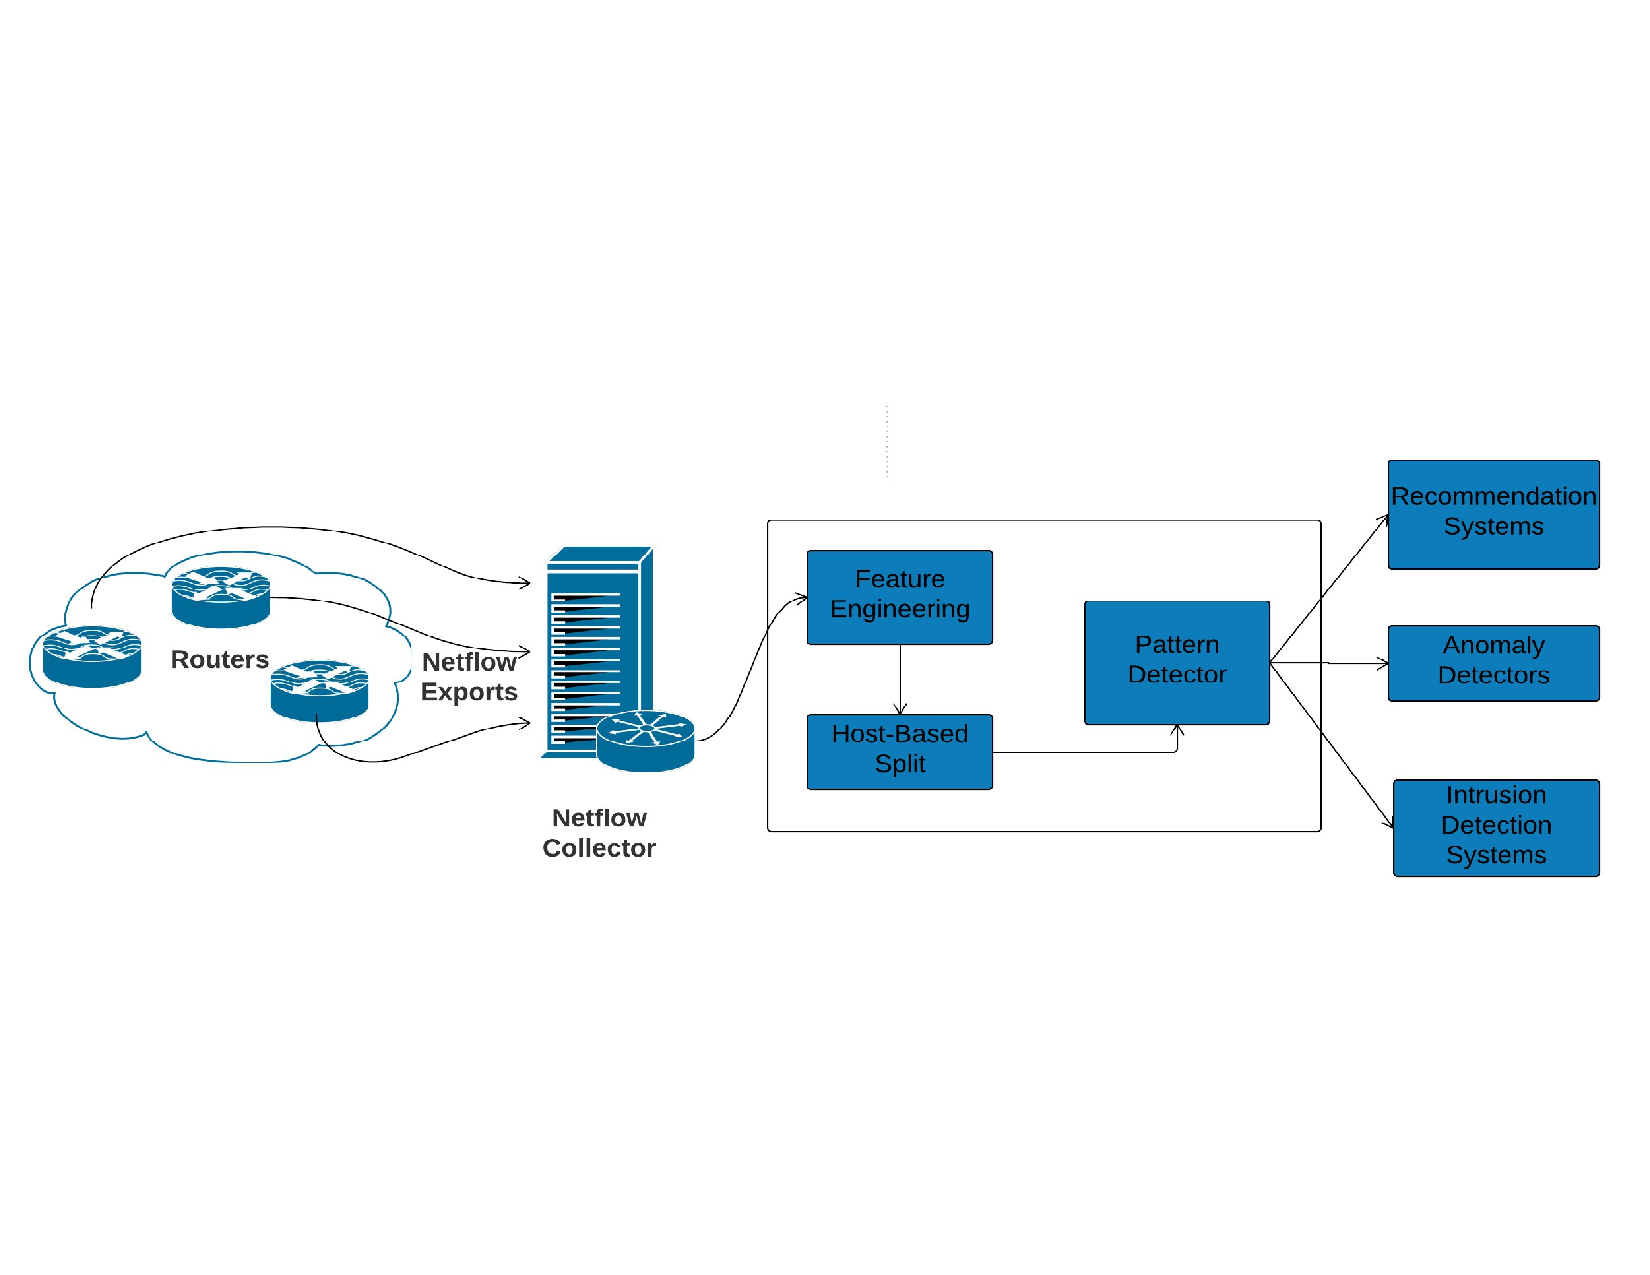
\includegraphics[trim=4cm 4cm 4cm 4cm, scale = 0.6]{architecture.pdf}}
	\caption{Architecture.}%
	\figlabel{arch}
\end{figure}

\subsection{NetFlow collection}
While the term NetFlow has become a de-facto industry standard, many other network hardware manufacturers support alternative flow technologies namely JFlow, S-Flow, NetStream, etc.. The University routers from which we have collected the data for this experiment have been equipped with NetFlow on it which led to using NetFlow as our flow technology. 
\subsubsection{What is NetFlow?}
NetFlow is a proprietary protocol for collecting IP flow packets information on networks. There are different variants to this protocol but across all these versions a flow is defined uniquely by its source and destination IP addresses, source and destination ports, transportation protocol. Whenever one of these values changes a new flow is created. For each flow the number of packets, bytes and other network related information are tallied and stored in the routers cache till it expires, then this information is exported to a collector. 

The captured flows are exported to NetFlow collectors at frequent intervals. The flows that are to be exported are determined based on the following rules: 1) When a flow is inactive for a certain time without receiving any new packets. 2) If the flow is active than max threshold time which is configurable. 3) If a TCP flag (FIN / RST) indicates the flow is terminated. NetFlow provides a powerful tool to keep track of what kind of traffic is going on the network and is widely used for network monitoring. Most vendors support similar flow monitoring techniques and IETF IPFIX working group does a common standardization.

There are different variants of NetFlow with each advanced version giving additional information about the flow. The fields that we used in our experiment and that are supported across the versions are in \figref{netflow}.

\begin{figure}[t]
	\centerline{
	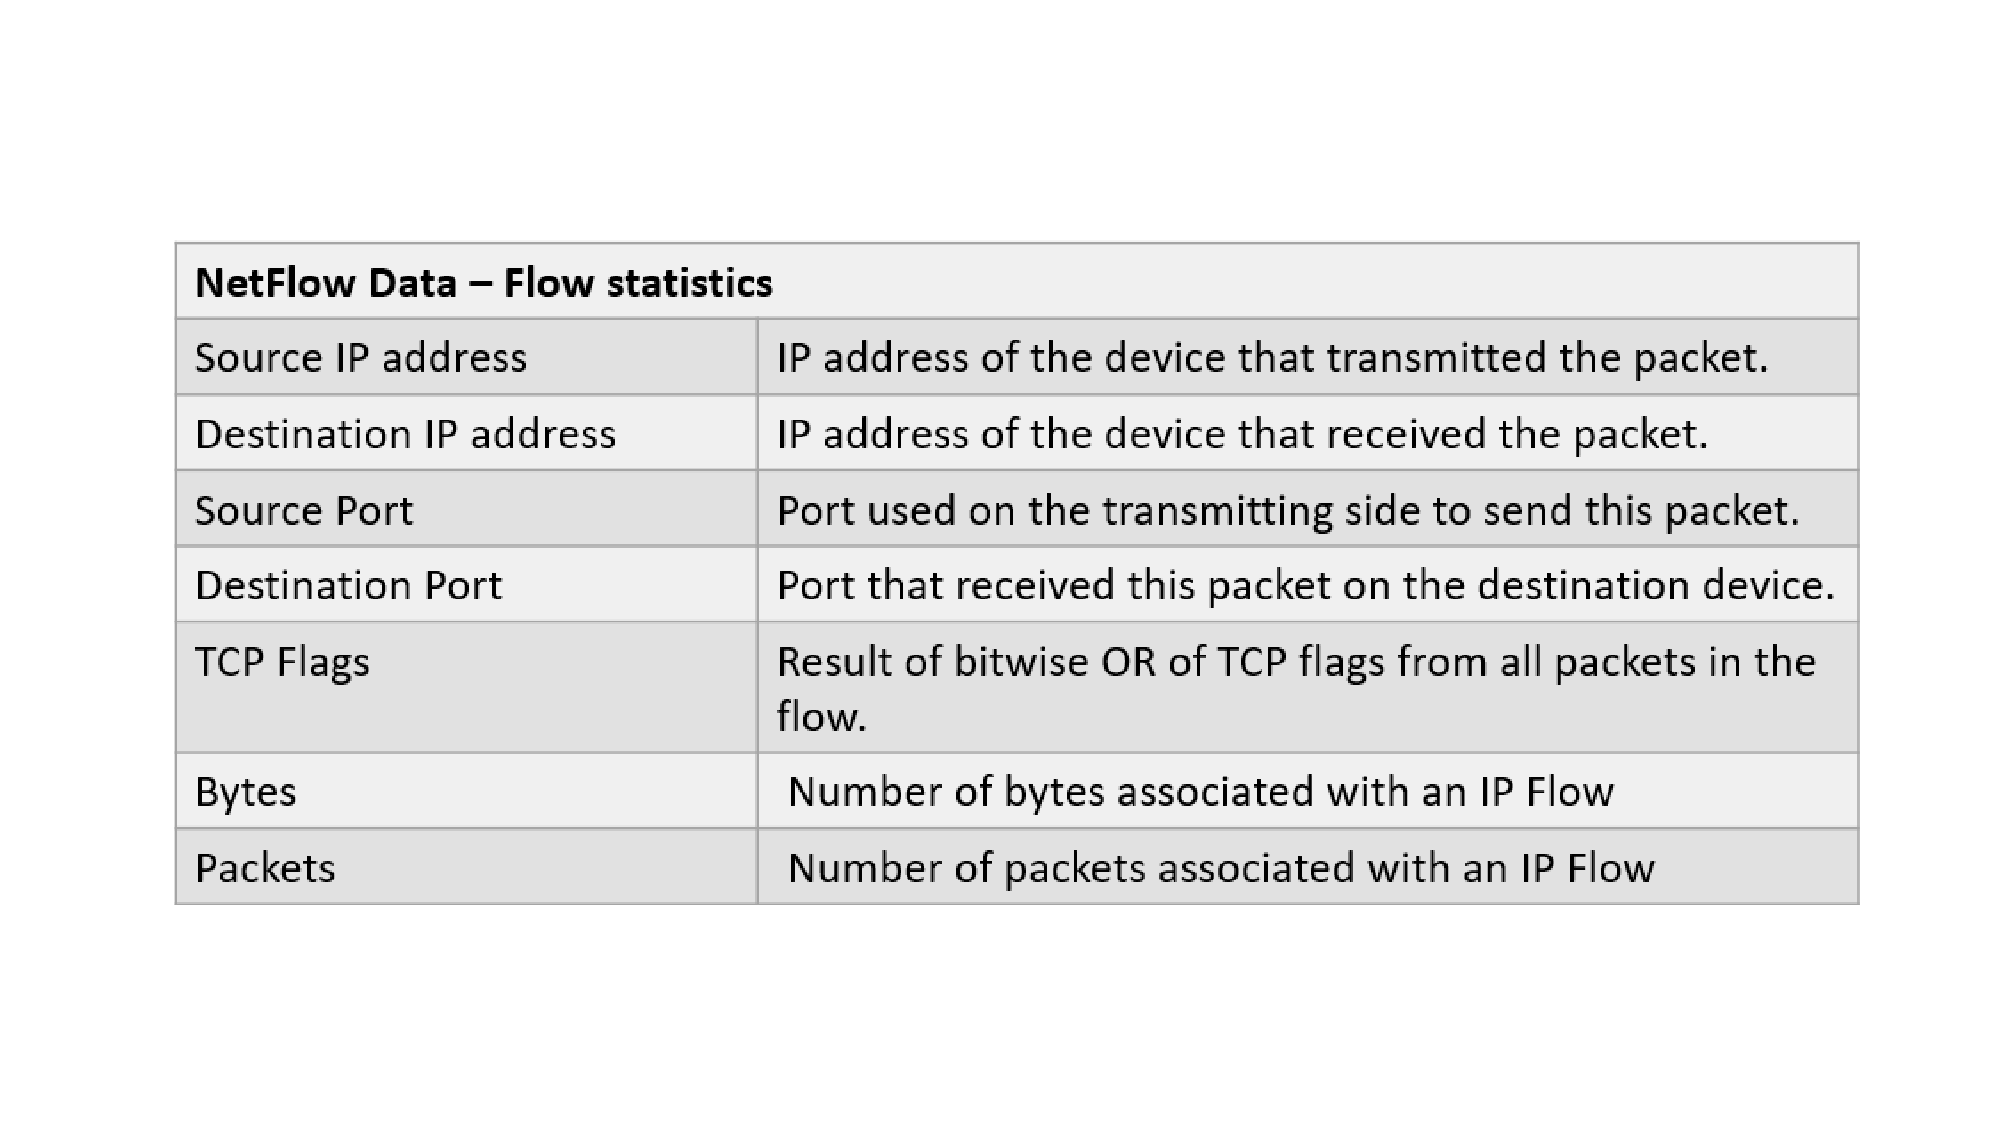
\includegraphics[trim=2cm 2cm 2cm 2cm, scale = 0.55]{netflow.pdf}}
	\caption{NetFlow fields captured in a Flow }
	\figlabel{netflow}
\end{figure}

\subsection{Feature Engineering}

Feature Engineering is the process of transforming raw
data into features so as to better represent the underlying structure of the data. This helps in increasing the accuracy of the models we build using data mining techniques. This step comes before modeling and after seeing the data.
Features extracted from the data directly influence the models generated and predictions made out of it. The better the features are the better the results will be. The results that we achieve when we are using DM approaches are a factor of the data set in hand, the features generated, the prediction model and the way the problem is framed. Most of the times even simpler models perform better if the features describe the structure inherent to the data. 
Below we describe different steps involved in the feature engineering with a sample set of data.
\begin{table}[t]
	\caption{Netflow raw data.}%
	\centerline{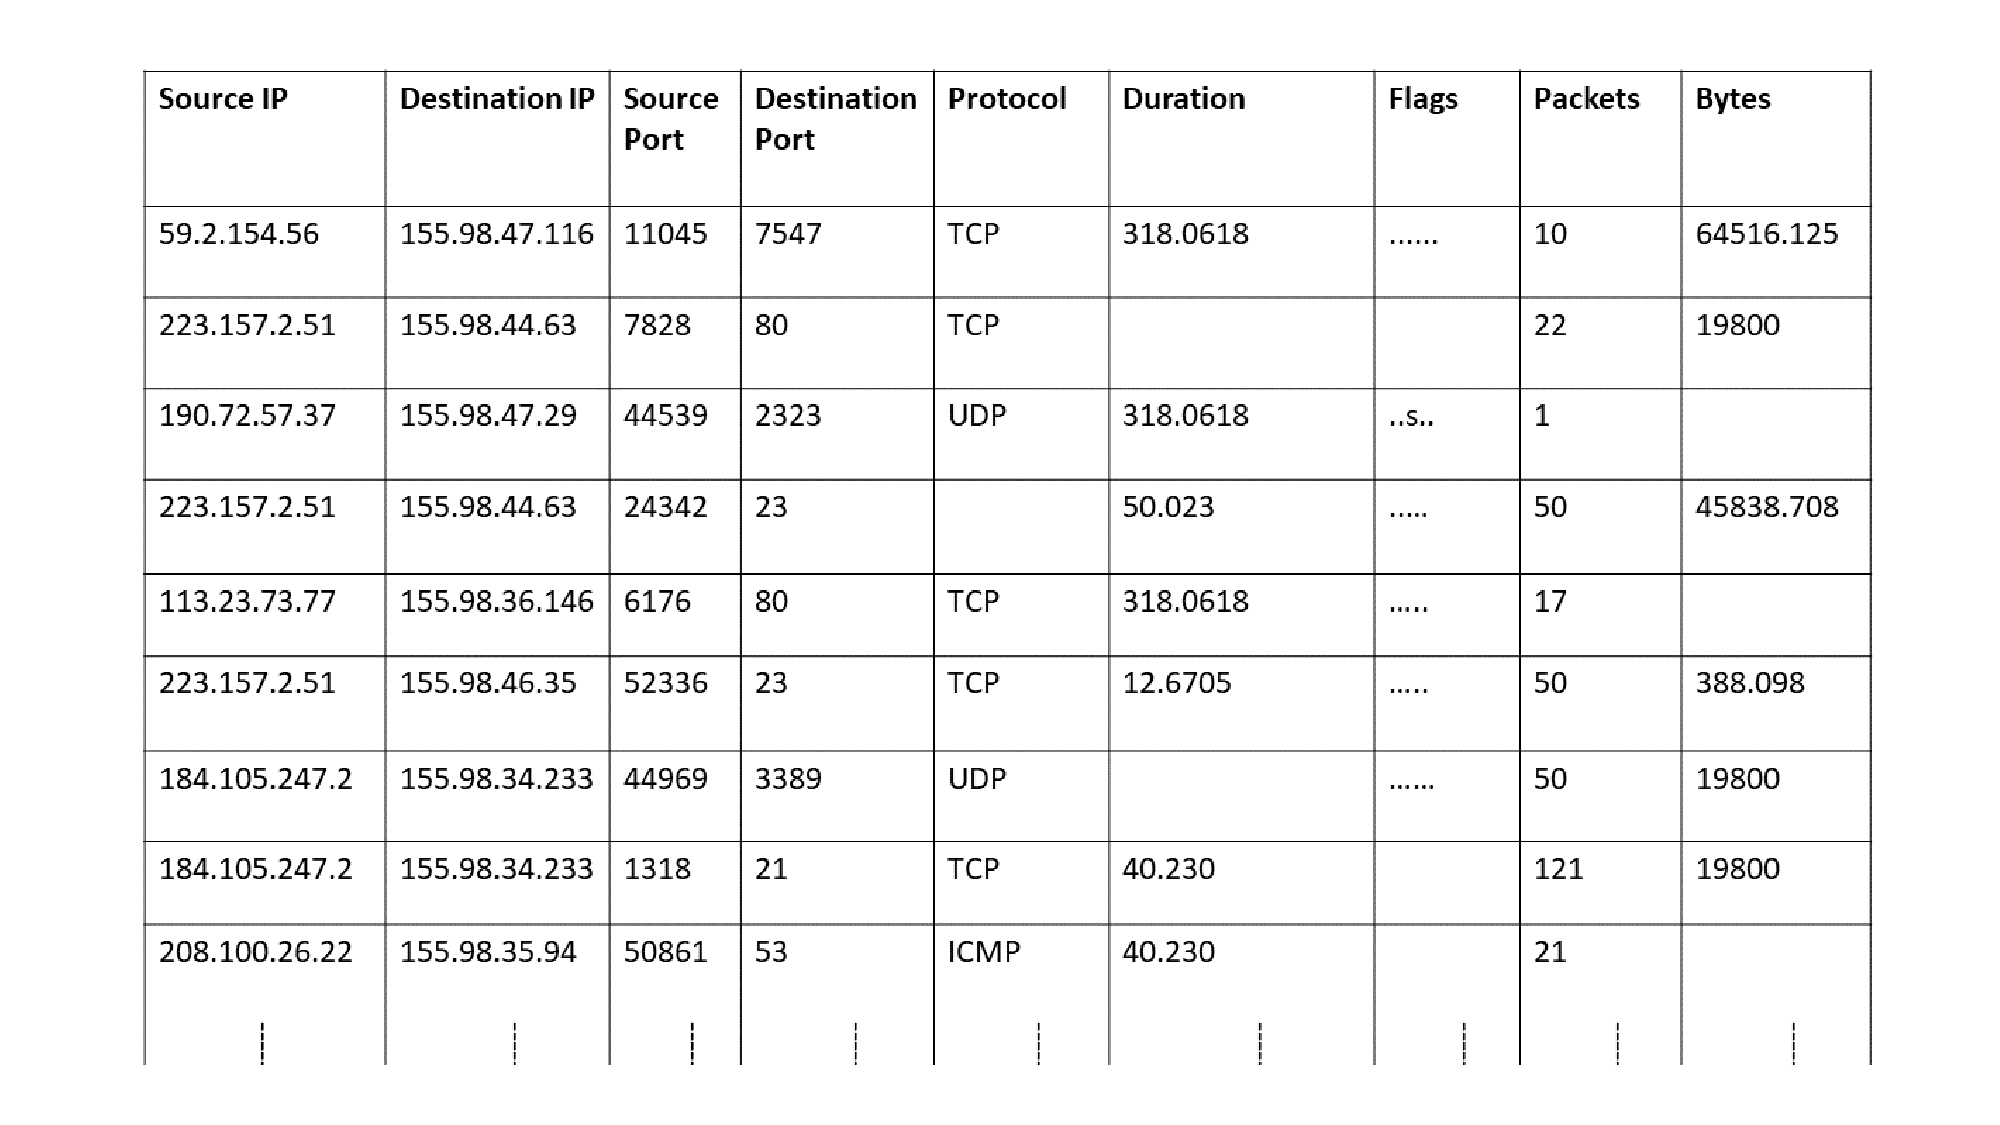
\includegraphics[scale = 0.5]{raw_data.pdf}}	
	 \tablabel{raw_data}
\end{table}
 
\subsubsection{Missing Data} 

\tabref{raw_data} is a sample of network data collected using NetFlow. In total there are 40 columns (only 9 columns are shown in the table) for each record with each column capturing different flow information. From the table, we can see that there are few missing values. Missing data is a common issue that every data science experiment has to deal with and there could be different reasons why NetFlow records could be missing some values such as, few filters could be turned on the router that doesn't let the NetFlow collector collect all the information, overloading of NetFlow collector and others. We handled Missing data using the following techniques 

1) Replace missing values with the mean. For the features such as duration, total packets and bytes exchanged we assume that missing values are distributed similarly to the values that are present for each source IP. The rational approach here would be to substitute values using mean as it maintains the existing distribution.

2) Replace missing values with the median/ mode. This is another technique to handle missing data, It should be noted that using different statistical measures to replace missing values yield different solutions. Features that have categorical data cannot be handled using mean or median and hence we approach mode to fill in their missing values. The feature protocols were handled using the mode approach, filling the missing values with the most frequently occurring protocol value for that source IP.

3) The question that arises when replacing missing values is what percentage of values can a feature miss atmost. For example, filling in half the values of a feature in this step with a statistical measure is not reasonable. Features of this kind are considered as noise and could affect the effectiveness of the data mining algorithm. The better option here would be to discard the column that has too may missing values. In our case, there were a handful of columns that fell under this category and are discarded. flags shown in \tabref{raw_data} is one among them. After handling missing values our data looks as in \tabref{missing_data}.

\begin{table}[t]
	\caption{NetFlow raw data after handling missing values}%
	\centerline{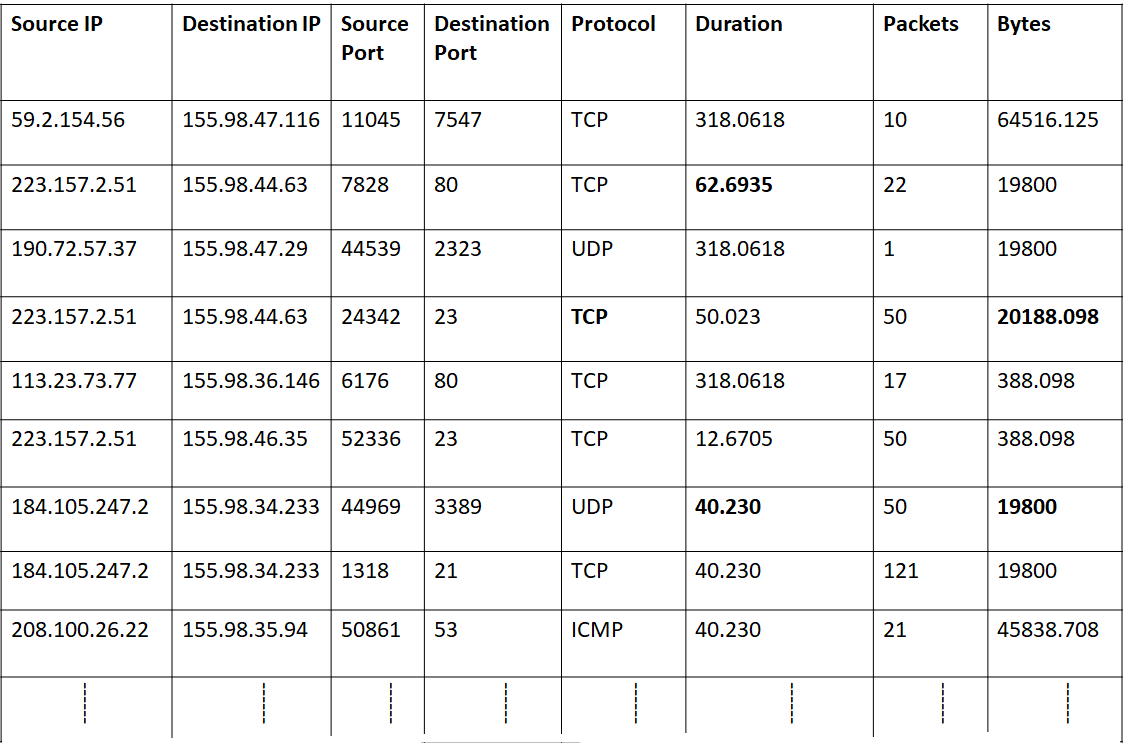
\includegraphics[scale = 0.6]{missing_data.png}}
	
	\tablabel{missing_data}
\end{table}


\subsubsection{Converting categorical to numerical variables} 

Features could be either numerical or categorical variables. When dealing with algorithms that work on numerical data we have to make sure that the categorical variables are handled.
For example, in our case feature protocol, has values such as TCP, UDP, and others. One approach is to encode them as 0, 1, and 2 respectively converting them to numerical variables. This could pose a problem when using distance measuring algorithms as the distance between the encoded attributes, like 1 (UDP), 0 (TCP) is smaller than 0 (TCP), 2 (others) generating an unintended meaning to this feature and could lead to biasing of few values. Another approach would be to create a feature for each value of the categorical variable and mark it as 0 or 1 based on if the value is present or not. There are both pros and cons to this method. The pros are if we choose to aggregate the values on all features this conversion gives a numerical value to work with. The cons are scaling and standardization could be affected. \tabref{categorical} represents data set after this step.

\begin{table}[t]
	\caption{After Converting categorical data to numerical}%
	\centerline{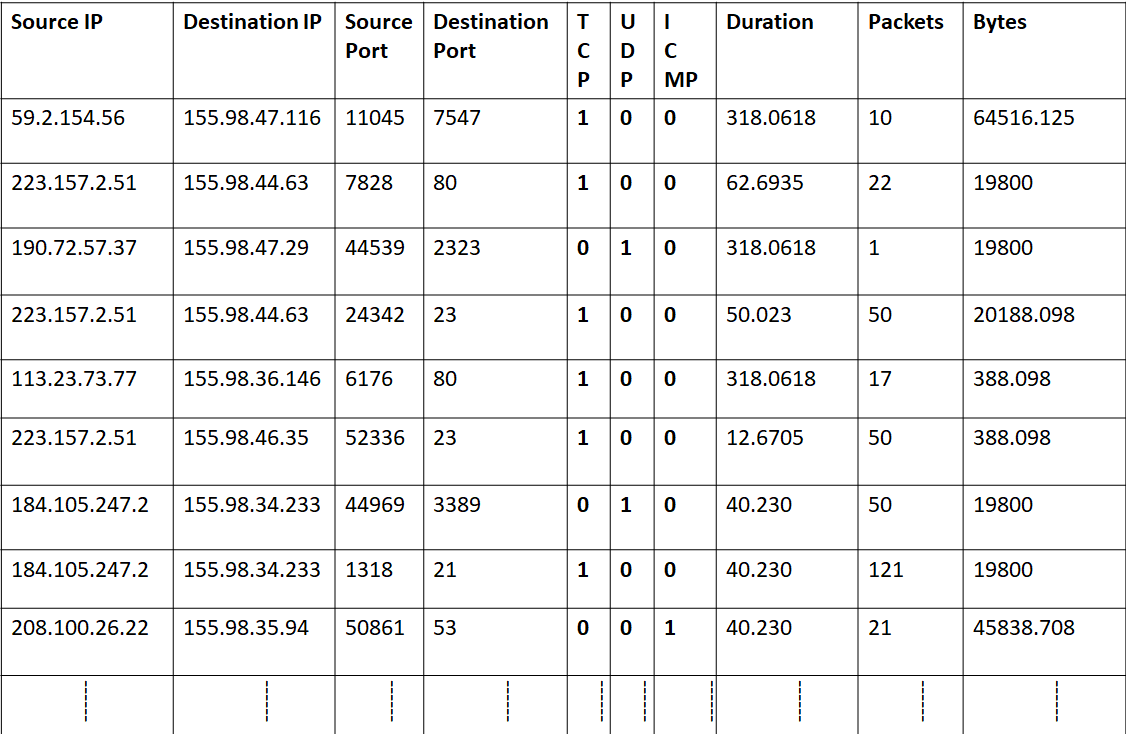
\includegraphics[scale = 0.6]{categorical.png}}
	\tablabel{categorical}
\end{table}

Above two steps fall under a family of techniques called data cleaning. After the data cleaning and removing the irrelevant columns of data using domain knowledge we aggregated NetFlow data based on source IP as our work focuses learning about hosts from their aggregate data. The \tabref{aggregated} shows a sample of aggregated data with ten features.
The first record in the \tabref{aggregated} conveys the information that in the given data set the host 59.2.154.56 (source IP) had appeared 450 times. Out of those 450 instances it had contacted 116 unique hosts. A total of 110 different source ports were used in the 450 flows and all the packets were sent to single destination port. The columns TCP, UDP, ICMP indicate how many of these flows fall under each category. So of the 450 flows there are 406 flows in which TCP protocol was used , 4 had UDP protocol used and the rest 40 had used ICMP protocol. And the columns Total Duration, Total Bytes, Total Packets indicate the respective information exchanged by this source IP on a whole. This aggregated data is what we use for learning host behaviors. But, before that, we have to apply few other feature engineering techniques as described below.

\begin{table}[b]
	\caption{Aggregated data by Source IP}%
	\centerline{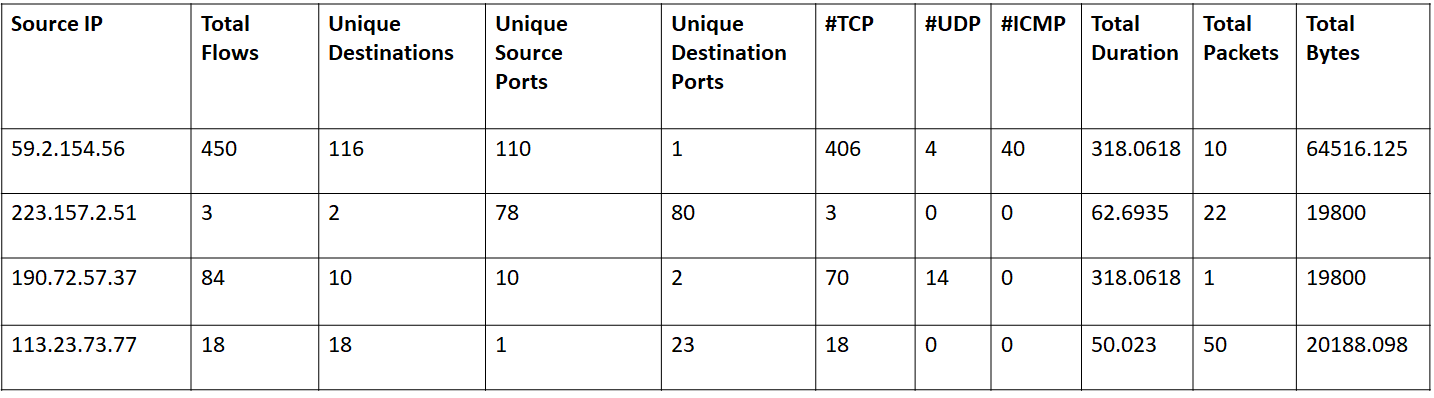
\includegraphics[scale = 0.6]{aggregated.png}}	
	\tablabel{aggregated}
\end{table}


\subsubsection{Feature scaling} 
Feature Scaling/Feature Normalization, a method used to standardize the range of independent features of data. Failure to standardize variables might result in algorithms placing undue significance to variables that are on a higher scale. For example from the \tabref{aggregated} it is evident that the total packets and total bytes have higher magnitude compared to total flows and destinations. This range difference shouldn't bias our results.
There are different ways to do feature scaling namely, Min-Max scaling, Variance scaling, L2 normalization etc.. The choice depends on the data and different statistics of it such as mean, variance, l2 norm. Scaling is not advisable in all instances we might lose valuable information if applied without proper thought. In our case, we have chosen simple Min-Max scaling as our goal was merely to change the range of the data and not the distribution and Min-Max scaling helps us in achieving this at a lower cost.

\subsubsection{Feature transformation} 
Transforming non-normal distribution to normal, many ML/DM tools perform well on normalized data and having skewed data will give inaccurate results. Log transformations are generally used to normalize the skewed data which is the case with most network data. After transforming the data if it doesn't capture the essence of original data we could look at other options such as square root, cube root. BoxCox is also another technique that changes the distribution of variables from non-normal to normal or near normal. \figref{feature} shows the distribution of a feature 'Total Flows' from our aggregated data, as seen from the graph it is heavily skewed towards left and this can be directly attributed to the data set we have in hand. The graph indicates that in most instances number of flows in which a source IP appears is less than 100 and hence we employ transformation techniques to decrease the amount of skewness in the data.  \figref{feature_transformed} shows the same data after applying log transformation. 

\begin{figure}[t]
	\centerline{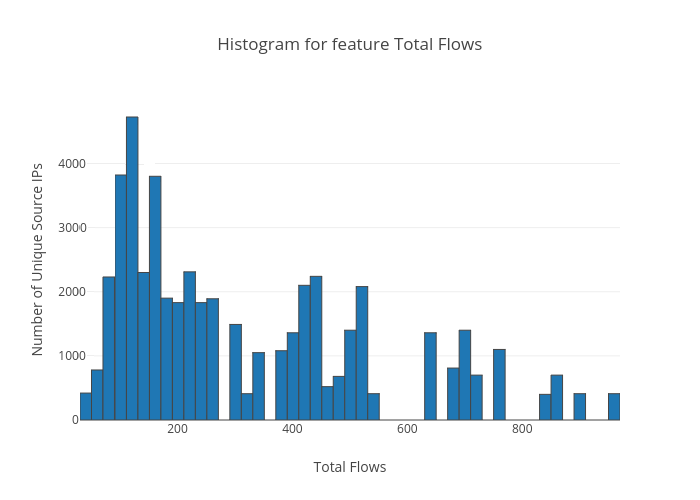
\includegraphics[scale = 0.9]{feature.png}}
	\caption{Skewed data before transformation}%
	\figlabel{feature}
\end{figure}

\begin{figure}[t]
	\centerline{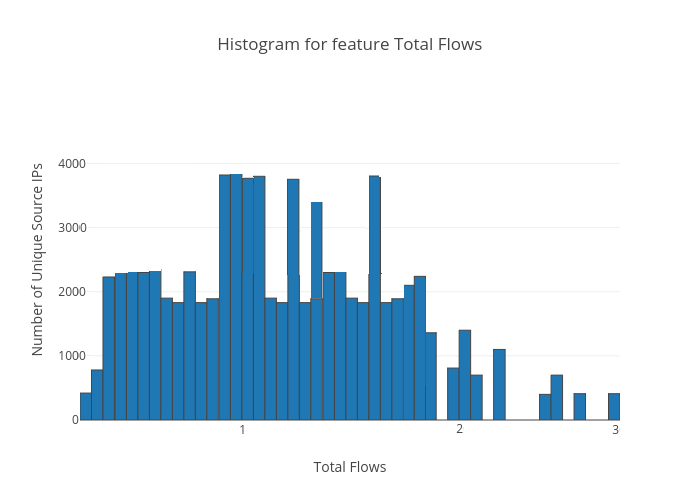
\includegraphics[scale = 0.9]{transformed.png}}
	\caption{Normalized data}%
	\figlabel{feature_transformed}
\end{figure}



\subsubsection{Feature selection}		
	
	Feature selection refers to the process of selecting a subset of relevant features to model the data. It helps in shorter time periods of execution, overcoming the overfitting problem and making the solution more generic and avoid the curse of dimensionality. The central premise of this process is to remove redundant or irrelevant features that don't make much sense to the problem we ought to solve. Feature selection and dimensionality reduction are two confusing terms. Though both methods seek to reduce the number of attributes in the dataset, but dimensionality reduction does it by creating new combinations of attributes, whereas feature selection methods include and exclude attributes present in the data without changing them. Principal Component Analysis, Singular Value Decomposition are examples of dimensionality reduction methods. The techniques used to do feature selection depend on text, numerical variables and they are three general classes of them Filter, Wrapper, Embedded methods.	Feature selection is a much tougher problem in unsupervised setting as we don't have any labels that help us in determining the information gain with and without a feature. Problems of
	this kind have been rarely studied in the literature \cite{boutsidis2009unsupervised} \cite{dash2002feature}. 
	
	The common strategy of most approaches is the use of filter methods, Filter model methods do not utilize any clustering algorithm to test the quality of the features. They evaluate the score of each feature according to criteria mentioned here \cite{dash2002feature}. It selects the features with the highest score. It is called filter since it filters out the irrelevant features using given criteria. 
	Wrapper methods are another class of methods used for feature selection where we train the given model with different combinations of features and make inferences accordingly.
	Some common examples of wrapper methods are forward feature selection, backward feature elimination. Forward selection is similar to elbow method explained in the next section. It is an iterative technique where we start with zero features and in each step, we keep adding feature that has the most information gain or best expresses the underlying structure. This procedure is stopped when addition of an extra feature doesn't add any significant information to the model. The backward elimination technique is exactly opposite to the forward selection method. Here we start with all the features and remove the feature with least information gain at each iteration. This iterative procedure stops when removal of features doesn't improve our model.
	
	We have chosen wrapper methods backward elimination technique for feature selection as it measures the usefulness of a subset of features by actually training a model on it. Though, it is computationally expensive compared to filter based approaches in our context it was reasonable as we had only 10 features to look into. The result of feature selection is we have detected two features that have very less information gain namely the ICMP ports and duration and hence we removed these two from our feature list making our final feature count to 8.
	 Feature Selection has helped us in enabling the machine learning algorithm to train faster. It reduced the complexity of the model and made it easier to interpret. We were also able to address the overfitting problem.






\section{Pattern detector}
Pattern detector consists of the core logic of our system. After cleaning the data and applying feature engineering we send the data through a pattern detector. Pattern detector sends the data through a clustering algorithm. It then maps the generated clusters to the host behaviors which is explained later.

As mentioned in the background section we choose to address our problem using unsupervised learning approaches. The most common unsupervised learning method is cluster analysis, which is used for exploratory data analysis to find hidden patterns or grouping in data. 

\subsection{Why K-Means ??}
 In section \ref{unsupervised} we have discussed the different type of clustering techniques in detail. Here we provide a reasoning for choosing K-Means.
 
Connectivity models like hierarchical clustering don't have a provision for relocating objects that may have been incorrectly grouped at an early stage. Also, use of different distance metrics for measuring distances between clusters may generate different results. Performing multiple experiments and comparing
the results is recommended to support the veracity of
the original results. Lastly, a time complexity of at least O($n^2logn$) is required, where n is the number of data points thus lacking scalability for handling big datasets.

Distribution Models assume a distribution for data but for many real data sets, there maybe no concisely defined mathematical model (e.g. assuming Gaussian distributions is a rather strong assumption on the data). Also, though distribution models have an excellent  theoretical foundation but they suffer from one key problem known as overfitting. 

We have experimented our data set with the density model DBSCAN and we have found the data being grouped at most into only two clusters. The reason for this is that density based models expect some kind of density drop to detect cluster borders. Recall from the above section that our dataset has many source IPs that appear in less than 100 flows and hence there wasn't any drop in density observed resulting in bad clustering.

Experimenting with centroid models especially K-Means gave us the advantage to play with the variable K and view into how hosts are being grouped with different values of K. It is scalable for heavier datasets and doesn't suffer from the overfitting problem. Also, there isn't any inherent assumption on which distribution the dataset should follow. Thus, making it a clear choice for building our system.


\subsection{How to choose K ??}
 In many situations, parameters and variables chosen by the algorithm or by users affects the performance of the algorithm differently and results in different outputs. Similarly, an essential problem of the K-means clustering method is to define an appropriate number of clusters K. In the literature, there are different approaches proposed to determine an accurate value of K.
 These methods include direct methods and statistical testing methods. Direct methods consist of optimizing a criterion, such as the within-cluster sums of squares or the average silhouette. The corresponding methods are named elbow and silhouette methods, respectively. Statistical testing methods consist of comparing evidence against the null hypothesis. An example is the gap statistic. We have used the direct methods as they optimize a criterion, The elbow method was used to determine K and then cross-verified the values with the Silhouette Index obtained for this same data set.
 
 From \ref{unsupervised}, it is clear that K-Means clustering tries to map a data point to the closest cluster center. Thus, it tries to minimize the total within-cluster sum of square (WSS). The total WSS measures how compact the formed clusters are and this has to be as small as possible. The elbow method that we used to determine K measures the total WSS for each value of K. We chose a K value(i.e, number of clusters) such that an increment or decrement of K value shouldn't improve the total WSS. 
 Steps in elbow method are outlined as follows:
 \begin{itemize}
 	\item Compute k-means clustering for different values of k. We used k value ranging from 1 to 50.
 	
 	\item For each k, calculate the total within-cluster sum of square ($WSS_k$).
 	\begin{center}
 	 	\boldsymbol{$D_k = \sum_{x_i \in C_k} \sum_{x_j \in C_k} ||{x_i -x_j}||^2$}	 \\
 	 	
 	 	
 	 	\boldsymbol{$ WSS_k = \sum_{1}^{K} \frac{1}{n_k} D_k$}
 	\end{center}  
    Where K is the number of clusters, $n_k$ is the number of points in cluster k and $D_k$ is the sum of distances between all points in the cluster.
 	\item Plot a curve with wss values on y-axis and corresponding k values on x-axis. 	
 	\item The location of a bend in the plot indicates the optimal number of clusters into which the given data has to be split into. The x-axis value at the bend is used for K.
 \end{itemize}

  \figref{elbow} shows the elbow curve obtained for our data set on a chosen day. We can observe from the graph that initial clusters added more information and this has dropped after a point, giving an angle in the graph. This x-value at this bent gives us the optimal value for K which turns out to be 7.
 	

\begin{figure}[b]
	\centerline{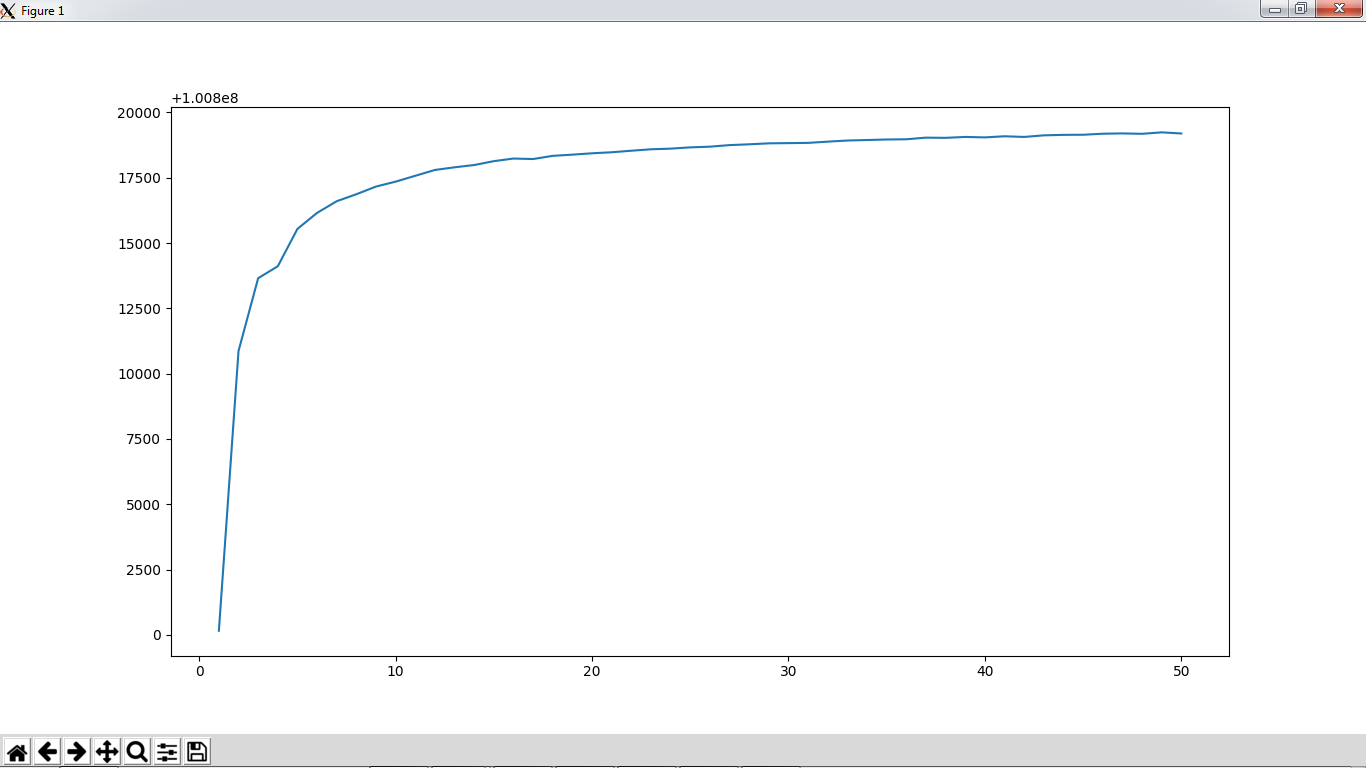
\includegraphics[scale = 0.4]{elbow.png}}
	\caption{Elbow Method}%
	\figlabel{elbow}
\end{figure}

 However, we cannot always rely on elbow method because it doesn't perform well if the data is not very clustered. Sometimes the plot doesn't have a bent instead it has a smooth curve. Hence, to overcome situations like this we also run our dataset through another technique called Silhouette to corroborate the claim of elbow method for K.
 
 Silhouette approach measures the quality of a clustering. We calculate silhouette value for each data point and find average silhouette value as explained below. Higher the average value higher is the quality of clustering. Similar to elbow method we calculate average silhouette value for different values of K. and chose the K for which this value is maximum. Steps involved in calculating silhouette value are as follows:
 	
		\begin{itemize}
		\item Run K-means clustering for different values of K. We used K value ranging from 1 to 50.
		\item Compute the average silhouette of observations for each K value (avg.sil).
		
		\begin{center}
			\boldsymbol{$s(i) = \frac{b(i) - a(i)}{max(a(i),b(i))}$}
		\end{center}
		Here s(i) is the silhouette index of a cluster point i. Where a(i) is the average distance of point i to all the objects in the same cluster while b(i) is the minimum average distance from the point i to all the points of a different cluster. avg.sil is calculated by finding the mean of all the s(i) for each point in a cluster.
		
		\item Plot the graph for avg.sil, with K value on x-axis and corresponding avg.sil value on y-axis.
		\item The peek of the graph is the optimal value for K.
	\end{itemize}
 
  The intuition behind this approach is for a point $i$, $ a(i)$ is  measure of how similar $i$ is to its own cluster, a small value of $ a(i)$ means it is well matched. Similarly, $b(i)$ is measure of how disimilar $i$ is to its own cluster, a larger value means $i$ is badly matched to its neighboring clusters. Thus a value of $s(i)$ that is positive and close to 1 indicates the point is correctly mapped. Further a negative value close to -1 indicates that it would be appropriate to group this point to its neighboring clusters. The average $s(i)$ on the whole data measures how tightly the data is grouped. Thus, higher avg.sil value defines that clusters formed are compact and of higher quality. \figref{silhouette} shows the plot obtained using silhouette technique. 
 
   An important point that has to be noted here is that, though we have a method to evaluate K, we don't invoke this method daily to determine the K value. We chose a reference day and determine the K value for that day and that K value is used for the remaining days till the network admin chooses to change this reference day. A reference day is selected generally to reflect all the behaviors that are seen in our network in day-to-day basis. The choice of changing this reference day also vests with the network admin as he knows how the usage of the network has been changed and whenever a reference day is changed we need to calculate the K value again.
   
 \begin{figure}[t]
 	\centerline{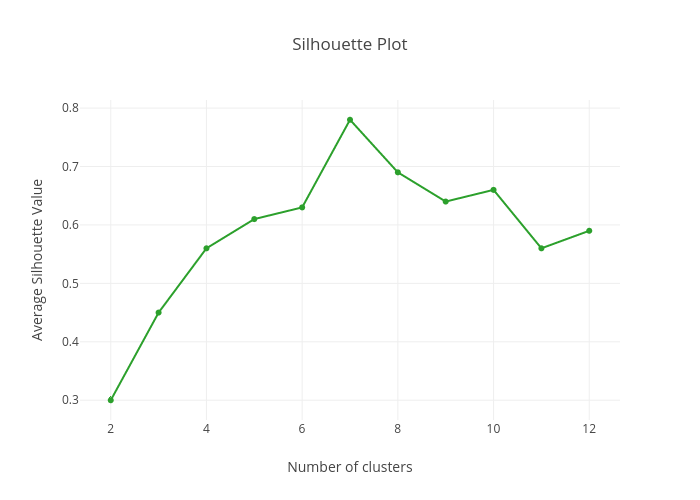
\includegraphics[scale = 0.6]{silhouette.png}}
 	\caption{Silhouette Method}%
 	\figlabel{silhouette}
 \end{figure}
 
\subsubsection{Cluster labeling and comparison}  \label{cluster_labeling}

The output of the pattern detection step is a set of clusters. We explored these clusters to better understand the grouping of hosts. We observed that each cluster exhibits a unique behavior. That is all the hosts in a cluster exhibit similar behavior. These clusters were labeled accordingly which is further discussed in evaluation chapter.
Recall the overarching premise of our work is to analyze the behavior of hosts looking at the aggregated host data. In order to analyze the behavior of hosts over a time period, we should be able to compare hosts behavior across days. We dealt with this by initially comparing the host's behavior for any two days and then extended it to any given time period. To achieve this we chose a reference day and label the clusters on that day through manual inspection. On any other day, we label the clusters by comparing it with this reference day. Cluster comparison is an active research area but in our case, it is slightly easier to solve because the number of clusters that are formed on each day is constant (i.e, as we choose the same K value as on reference day.) and each cluster maps to a unique behavior. So, all that we need to do is to find a one-to-one mapping with the reference day clusters. 
Now, this turns out to be an assignment problem which is well studied \cite{kuhn1955hungarian}. Assignment problem is a special type of linear programming problem which deals with the allocation of the various resources to the various activities on one to one basis. It does it in such a way that the cost or time involved in the process is minimum and profit or sale is maximum. 

In our case both the resources and activities are nothing but clusters formed on two different days and this has to be done in such a way that the total effort is least. Assignment problem is a well-studied problem and has polynomial time solutions. One such algorithm is the Hungarian algorithm\cite{kuhn1955hungarian}.

\section{Applications} \label{applications}
Our system can be used to build different applications that help in network management as listed below.
\begin{itemize}
	
	\item \textit{Anomaly Detectors}, applications that expose the hosts that are behaving as outliers and don't conform to an expected pattern. We can use our system to build such applications. For example, we found a cluster of hosts that are exhibiting anomalous behavior during our exploration of  emulab data. We can observe the change of this cluster size and center over days and thereby notifying the network admin if there is a shift in anomaly behavior that network admin has to be aware of. Here we can take the help of  work done by \cite{DBLP:journals/corr/DeyRS17} to determine when should a network admin be notified. 
	
	\item \textit{Dynamic Security Rules Generator}, Looking at the historic user behavior we can generate dynamic rules for security of the network. Few of them could be, to block certain IPs that are exhibiting inconsistent behavior etc. Authentication rules can also adapt dynamically by observing the changes of different clusters and their cluster centers. Such as, number of unsuccessful attempts a client can make to a server can also be limited based on the different ports client is using.
	
	\item \textit{Recommendation Systems}, We can capture the different behaviors exhibited by network users over time and use this to predict a behavior on a certain day of a week or month using the historical data. This helps network admin to prepare well ahead and plan the bandwidth or other network resources accordingly.
	
	In this direction of building applications through the results obtained from our system we have created a web tool that analyzes data in different dimensions and is explained in detail in evaluation chapter.

\end{itemize}


 

%In that direction of building a recommendation system we came up with an user interface that helps to analyze historic data , this should go into evaluation section.%



